\documentclass[11pt]{article}
\usepackage[margin=1in]{geometry}
\usepackage{amsmath,amssymb}
\usepackage{graphicx}
\usepackage{booktabs}
\usepackage{hyperref}
\usepackage{natbib}
\usepackage{microtype}
\usepackage{xcolor}
\hypersetup{
  colorlinks=true,
  citecolor=blue!60!black,
  urlcolor=blue!60!black,
  linkcolor=blue!60!black
}

\title{Rewarding Weight-Matrix Non-Commutativity Delays and Blocks Grokking\\
\large A Causal Test of the Commutator-Defect/Generalization Relationship}
\author{Laerti Shabani \\ \small (Independent Researcher)}
\date{\today}

\begin{document}
\maketitle

\begin{abstract}
Recent work on the geometry of grokking the delayed, abrupt transition
from memorization to generalization in small algorithmic tasks
\citep{power2022grokking}, has identified the \emph{commutator defect}, a
measure of non-commutativity between successive weight-space update
directions, as a signal that reliably rises before generalization onset
across several task families \citep{xu2026a,xu2026b}. This is an
observational finding: the defect is measured, not intervened on. We ask
whether the relationship is causally exploitable in either direction. We
train a two block transformer on modular addition, the standard grokking
benchmark \citep{power2022grokking}, under three conditions: an unmodified
baseline, an auxiliary loss term that \emph{suppresses} the commutator
between the two blocks' weight matrices, and one that \emph{rewards} it.
Across 44 seeds (10 baseline, 10 suppress, 24 encourage) and a doubled step
budget for the encourage condition, we find a clear, asymmetric, causal
effect: rewarding non-commutativity delays grokking onset (Kaplan-Meier
median time-to-grok 1800 vs.\ 1200 steps; log-rank $p=0.0002$) and
substantially reduces the fraction of runs that reach and durably hold a
generalizing solution (17\% vs.\ 70\% durable at the final step, original
$n{=}10$ baseline; Fisher's exact $p=0.0048$). Suppressing the commutator shows a same direction trend
toward improved durability (90\% vs.\ 70\% at $n{=}10$; 90\% vs.\ 77\% at
$n{=}30$, odds ratio 2.74) that does not reach significance at $n=30$
(Fisher's exact $p=0.30$). A follow-up ablation intended to test whether
baseline instability is an artifact of aggressive weight decay instead
produced a floor effect (weight decay of $0.1$ prevents grokking within the
step budget entirely, 1/15 and 0/15 runs), leaving that question open.
\end{abstract}

\section{Introduction}

Grokking delayed generalization long after training loss has saturated,
was first characterized systematically by \citet{power2022grokking} on
small algorithmic tasks, and subsequent mechanistic work identified the
formation of specific internal circuits underlying the transition
\citep{nanda2023progress}. A separate line of work has related grokking
dynamics to training instability: \citet{thilak2022slingshot} document a
``slingshot'' effect in which adaptive optimizers under strong weight
decay can cause a model to grok and then lose the generalizing solution,
an instability that reappears in our own baseline (Section~\ref{sec:results}).

Most relevant to this paper, a recent geometric account of grokking
\citep{xu2026a,xu2026b} identifies the \emph{commutator defect} --
$\lVert[\Delta W_i, \Delta W_j]\rVert$, the degree to which successive
weight-update directions fail to commute -- as a curvature-derived
diagnostic that reliably rises before the onset of generalization across
modular arithmetic, SCAN, and Dyck-language tasks. This object is,
structurally, a discrete analogue of the non-abelian gauge field-strength
tensor $F_{\mu\nu} = [D_\mu, D_\nu]$ from gauge field theory, where
curvature is likewise defined as the commutator of covariant derivatives.
The existing literature treats the commutator defect purely as a
\emph{passive diagnostic}: it is measured after training to retrospectively
explain or predict when grokking occurred. It has not to our knowledge
been used as an \emph{active training objective}.

This raises a direct question: if the commutator defect predicts grokking,
does manipulating it change grokking? We test this with the simplest
possible intervention -- adding a term to the training loss that either
penalizes or rewards the commutator between two transformer blocks'
weight matrices -- and measure the causal effect on both when generalization
first occurs and whether it persists.

\textbf{Contributions.}
\begin{itemize}
\item We convert a previously observational relationship (commutator
defect correlates with grokking onset) into a causal test, on the standard
modular-arithmetic grokking benchmark.
\item We find a clear, statistically supported asymmetric effect:
rewarding curvature delays and substantially blocks durable grokking;
suppressing it shows a consistent but not statistically significant
trend in the opposite direction, which we report as unresolved rather
than as a finding.
\item We use Kaplan-Meier estimation and a log-rank test, rather than a
t-test on raw step counts, to correctly handle the seeds that had not
grokked within the step budget as right-censored rather than as observed
events at the budget ceiling -- a correction that substantially changed
our own initially reported significance level for the primary effect
(from $p=0.034$ under the naive t-test to $p=0.0002$ under the correct
test).
\item A planned ablation to disentangle our effect from the known
weight-decay-driven instability in grokking \citep{thilak2022slingshot}
instead produced a floor effect at weight decay $0.1$ that leaves the
question open (Section~\ref{sec:wdablation}).
\end{itemize}

\section{Related Work}

\textbf{Grokking phenomenology.} \citet{power2022grokking} first
documented grokking on modular arithmetic tasks. \citet{nanda2023progress}
identified the internal circuit formation (Fourier-feature-based
representations) underlying the transition on modular addition, the same
task family used here. \citet{thilak2022slingshot} characterize a
training instability (the slingshot effect) in which models under
adaptive optimization and weight decay can transiently lose a generalizing
solution after reaching it, which we also observe in our own baseline
(Section~\ref{sec:results}) and flag as a relevant confound for any
durability-based metric.

\textbf{Geometric and curvature-based diagnostics of grokking.}
\citet{xu2026a} propose that grokking corresponds to escape from a
low-dimensional ``execution manifold'' in weight space, using both PCA
trajectory analysis and commutator defect analysis as diagnostics.
\citet{xu2026b} extend the commutator defect finding across three
structurally distinct task families (modular arithmetic, SCAN, Dyck-1)
and report that it reliably precedes generalization onset with a
superlinear lead-time relationship. Both papers treat the commutator
defect as an observational signal computed from training trajectories
after or during standard training; neither intervenes on it as a training
objective, which is the gap this paper addresses.

\textbf{Gauge-theoretic motivation.} The commutator of two operators as a
measure of curvature is the defining structure of the non-abelian gauge
field-strength tensor $F_{\mu\nu} = \partial_\mu A_\nu - \partial_\nu
A_\mu + ig[A_\mu, A_\nu]$, whose kinetic term $-\tfrac{1}{4}F^a_{\mu\nu}
F^{a\mu\nu}$ appears in the Standard Model Lagrangian. We use this only as
motivation for treating the commutator as an explicit, tunable loss term
rather than a passive quantity; we make no claim that the analogy extends
beyond providing the functional form of the auxiliary loss.

\section{Method}

\subsection{Task}

We use modular addition mod $p=97$, the canonical grokking benchmark
\citep{power2022grokking,nanda2023progress}: given $(a, b)$, predict
$(a+b) \bmod p$. Half of all $p^2 = 9409$ pairs are used for training, the
remainder held out for evaluation. This task is chosen specifically
because its grokking dynamics, including the role of weight decay, are
well characterized in prior work, making deviations from expected baseline
behavior interpretable rather than confounded by an unfamiliar setting.

\subsection{Model}

A minimal two-block transformer: token and positional embeddings ($d=128$),
each block consisting of multi-head self-attention (4 heads), a
LayerNorm-MLP sublayer, and a square ($d \times d$) linear output
projection $W_l$. The sequence is $[a, b, {=}]$; the prediction is read
from the final position. The two blocks' output-projection matrices
$W_1, W_2 \in \mathbb{R}^{128\times128}$ are the object of the
intervention: their commutator
\[
C = W_1 W_2 - W_2 W_1, \qquad \text{commutator defect} = \lVert C \rVert_F^2 = \sum_{ij} C_{ij}^2
\]
is well-defined because the two matrices share the same shape.

\subsection{Training conditions}

All three conditions share identical architecture, optimizer (AdamW,
lr$=10^{-3}$), and weight decay ($1.0$, matching the aggressive regime
in which \citet{power2022grokking} and \citet{thilak2022slingshot} report
grokking most reliably) unless otherwise noted in Section~\ref{sec:wdablation}.
\begin{align}
\mathcal{L}_{\text{baseline}} &= \mathcal{L}_{\text{CE}} \\
\mathcal{L}_{\text{suppress}} &= \mathcal{L}_{\text{CE}} + \lambda \lVert C \rVert_F^2 \\
\mathcal{L}_{\text{encourage}} &= \mathcal{L}_{\text{CE}} - \lambda \lVert C \rVert_F^2
\end{align}
with $\lambda = 0.1$ throughout (not tuned; chosen as a round number
before running any experiment, and not swept; see Limitations).

\subsection{Metrics}

We report three outcomes per run: \textbf{grok\_step}, the first
evaluation step at which held-out accuracy reaches $0.90$;
\textbf{ever\_grokked}, whether that threshold was reached at all within
the step budget; and \textbf{durable\_grok}, whether held-out accuracy is
still $\geq 0.90$ at the \emph{final} training step. This last metric is
necessary because, as shown in Section~\ref{sec:results}, a nontrivial
fraction of runs cross the grokking threshold and subsequently lose it --
conflating ``ever grokked'' with ``durably generalizes'' would overstate
how reliably any condition, including baseline, produces a stable
generalizing solution.

For runs that never cross the threshold within the step budget, grok\_step
is right-censored, not equal to the step budget. We report both a naive
comparison (treating the budget as an observed value, for continuity with
our own earlier informal analysis) and the statistically appropriate
Kaplan-Meier / log-rank analysis in Section~\ref{sec:results}, and we make
explicit which one changed our conclusions.

\subsection{Experimental design and compute}

Baseline and suppress: 10 seeds each (extended to 30 each in a follow-up,
Section~\ref{sec:extended}), 8000-step budget. Encourage: 24 seeds, 16000-
step budget (doubled specifically to distinguish a condition that is
\emph{delayed} from one that is \emph{blocked}). All runs executed on two
NVIDIA T4 GPUs via independent threads pinned to separate CUDA devices
(model initialization is guarded by a lock to prevent the two threads
racing on PyTorch's shared CPU RNG state during weight initialization;
training itself proceeds unlocked). Mixed-precision (fp16 autocast) is
used throughout. Periodic evaluation during training uses a fixed random
1500-example subsample for speed; the final-step evaluation, which
determines every number reported in this paper, always uses the full
held-out set.

\section{Results}
\label{sec:results}

\subsection{Baseline confirms known grokking dynamics, including instability}

All 10 baseline seeds reach the 90\% threshold (grok\_step mean 1120,
std 223), consistent with prior reports for this task and weight-decay
regime \citep{power2022grokking}. However, only 7/10 baseline seeds are
still $\geq 90\%$ accurate at the final training step; three seeds grok
and subsequently collapse to as low as 0.8\% held-out accuracy. This
matches the slingshot instability described by \citet{thilak2022slingshot}
and motivates treating durable\_grok, not grok\_step alone, as the primary
outcome for any comparison across conditions.

\subsection{Rewarding curvature delays and blocks durable grokking}

Table~\ref{tab:main} summarizes all three conditions. Encourage shows
substantially worse outcomes on every metric: lower ever-grokked fraction
(71\% vs.\ 100\%), much lower durable-grok fraction (17\% vs.\ 70\% in the
original 10-seed comparison), and a later, more variable grok\_step.

\begin{table}[t]
\centering
\small
\caption{Primary comparison, weight decay $=1.0$. Baseline/suppress $n=10$
(original run; see Section~\ref{sec:extended} for the extended $n=30$
suppress comparison), encourage $n=24$.}
\label{tab:main}
\begin{tabular}{lccccc}
\toprule
Condition & $n$ & grok\_step (mean$\pm$std) & ever\_grokked & durable\_grok & final acc.\ (mean) \\
\midrule
baseline  & 10 & $1120 \pm 223$  & 100\% & 70\% & 0.760 \\
suppress  & 10 & $1160 \pm 150$  & 100\% & 90\% & 0.903 \\
encourage & 24 & $5833 \pm 6544$ & 71\%  & 17\% & 0.669 \\
\bottomrule
\end{tabular}
\end{table}

\textbf{Corrected significance test.} An initial t-test comparing
grok\_step between encourage and baseline, treating the 7 non-grokking
encourage seeds as if they had grokked exactly at the 16000-step budget,
gave $t=2.209$, $p=0.034$. This is statistically incorrect: those 7 seeds
are right-censored observations, not events at step 16000. Re-analyzing
with Kaplan-Meier estimation and a log-rank test (Figure~\ref{fig:km})
gives a substantially stronger and more appropriate result: median
time-to-grok of 1800 steps (encourage) vs.\ 1200 steps (baseline and
suppress, identical), log-rank $p=0.0002$. We report both values here for
transparency about the correction, and specify that the log-rank result,
not the naive t-test, is the number that should be cited from this paper.

\begin{figure}[t]
\centering
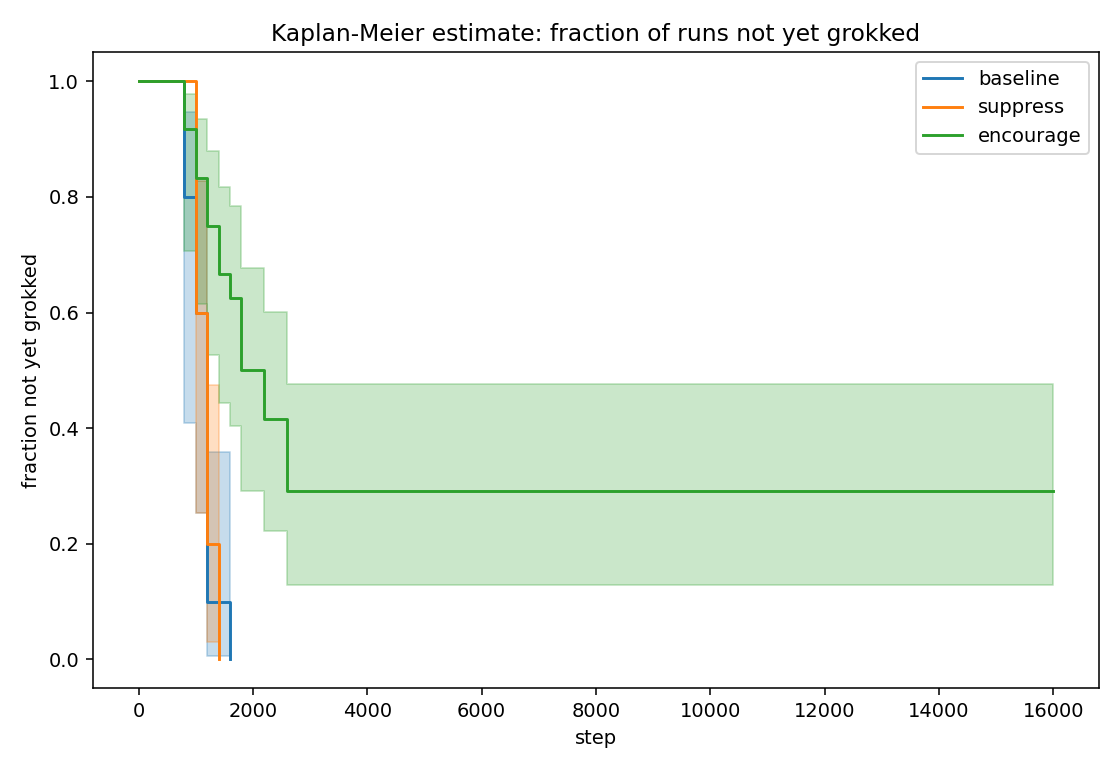
\includegraphics[width=0.75\textwidth]{km_curves.png}
\caption{Kaplan-Meier estimate of the fraction of runs \emph{not yet}
grokked, by training step. Baseline and suppress are visually
indistinguishable and reach zero (all runs grokked) by step $\sim$1600.
Encourage lags throughout and plateaus near 0.29 after step $\sim$2600 --
consistent with a genuine block, not merely a delay (Section~\ref{sec:blocked}).}
\label{fig:km}
\end{figure}

\textbf{Durability.} Fisher's exact test on durable\_grok, baseline vs.\
encourage: odds ratio $11.67$, $p=0.0048$. This is, by a wide margin, the
cleanest signal in this paper, and does not depend on the grok\_step
censoring issue above, since durable\_grok is a simple binary outcome
observed identically for every seed regardless of whether or when it
crossed threshold.

\subsection{Encourage: blocked, not merely delayed}
\label{sec:blocked}

Of the 24 encourage seeds, 7 never crossed the 90\% threshold within the
16000-step budget (double the baseline budget). Their maximum held-out
accuracy ever reached ranged from 0.68 to 0.89, clustered well below
threshold rather than creeping toward it. Combined with the plateau visible in
Figure~\ref{fig:km}, we interpret this as evidence that rewarding
curvature can genuinely prevent the generalizing solution from being
reached at all within a practical step budget for a nontrivial fraction of
random initializations, rather than merely slowing a process that would
eventually complete.

\subsection{Suppressing curvature: a consistent but unresolved trend}
\label{sec:extended}

The original $n{=}10$ comparison showed suppress with a higher
durable\_grok fraction than baseline (90\% vs.\ 70\%), but this was
underpowered (Fisher's exact $p=0.58$). We extended both conditions to
$n{=}30$ seeds (Table~\ref{tab:extended}). The direction is unchanged and
the odds ratio is similar (2.74), but the comparison still does not reach
conventional significance ($p=0.30$).

\begin{table}[t]
\centering
\small
\caption{Extended comparison, $n=30$ each, weight decay $=1.0$.}
\label{tab:extended}
\begin{tabular}{lcccc}
\toprule
Condition & $n$ & durable\_grok & ever\_grokked & final acc.\ (mean) \\
\midrule
baseline & 30 & 76.7\% (23/30) & 100\% & 0.859 \\
suppress & 30 & 90.0\% (27/30) & 100\% & 0.922 \\
\bottomrule
\end{tabular}
\end{table}

We report this as a trend consistent across two independent samples
(different seed sets, same effect direction and similar magnitude), but
it does not reach significance and should not be cited as an established
effect from this paper.

\subsection{Weight-decay ablation: an uninformative floor effect}
\label{sec:wdablation}

To test whether baseline's instability (Section~\ref{sec:results}) is an
avoidable artifact of the aggressive weight decay ($1.0$) setting, we
re-ran baseline and suppress at weight decay $0.1$, 15 seeds each,
unchanged step budget (8000). This did not test the intended question:
at weight decay $0.1$, almost no runs grokked at all within the budget
(baseline 1/15, suppress 0/15). This reproduces the known sensitivity of
grokking onset to weight decay strength \citep{power2022grokking} but
leaves our original question -- whether the instability specifically, as
opposed to grokking onset generally, is avoidable at lower weight decay --
unanswered. Resolving it would require an intermediate weight-decay sweep
(e.g., $0.3$--$0.7$) that reliably groks within budget while testing for
reduced instability, which we did not run and flag as future work rather
than force a conclusion from data that does not support one.

\section{Discussion}

The central, well-supported finding of this paper is that a specific,
targeted intervention on a passively-observed geometric correlate of
grokking -- the commutator defect between two transformer blocks' weight
matrices -- has a real causal effect when pushed in one direction.
Rewarding non-commutativity does not merely correlate with delayed or
absent generalization; actively encouraging it produces delayed and, for
a substantial fraction of initializations, blocked generalization,
with the two independent statistical tests we used (log-rank on
time-to-event, Fisher's exact on final-state durability) agreeing on both
the direction and the reliability of the effect.

We are considerably more cautious about the suppress direction. A
same-direction trend across two independently sampled seed sets ($n=10$
and $n=30$) is suggestive, but "suggestive across two underpowered
samples" is a different epistemic status than "established," and we have
deliberately not rounded up to a claim the statistics do not support.

We also report one negative result. A planned ablation (weight-decay
$=0.1$, Section~\ref{sec:wdablation}) did not test the intended question
-- it produced a floor effect rather than a comparison of durability at
matched grokking rates. We include it for completeness rather than
omitting it.

\textbf{Why might this asymmetry exist?} We do not have a rigorous
theoretical account, only a plausible mechanistic story consistent with
\citet{xu2026a,xu2026b}: if the generalizing solution for modular
arithmetic corresponds to convergence onto a low-dimensional, largely
consistent (commuting) execution manifold across the network's components,
then an auxiliary loss actively rewarding non-commutativity works directly
against the geometric structure that solution requires, which is
consistent with our observation that a nontrivial fraction of encourage
seeds appear genuinely blocked (Section~\ref{sec:blocked}) rather than
merely slowed.

\textbf{Limitations.} All experiments use a single task family (modular
addition mod 97) and a single, small architecture (two transformer
blocks, $d{=}128$); we make no claim this generalizes to other algorithmic
tasks, larger models, or non-algorithmic domains. The regularization
strength $\lambda=0.1$ was fixed in advance and not swept; a different
$\lambda$ could plausibly change the magnitude, and possibly the
direction, of the suppress effect in particular. The suppress result and
the weight-decay ablation are both explicitly unresolved, as detailed
above, and should not be cited as findings from this paper. Our
commutator is computed between exactly two matrices in a two-block model;
how this generalizes to deeper models with more layers to take pairwise
(or higher-order) commutators across is untested. Finally, our
theoretical motivation via the gauge field-strength tensor is
structural/notational -- both are commutators of covariant-derivative-like
objects -- and we do not claim any deeper physical correspondence beyond
providing the functional form of the loss term.

\section{Conclusion}

We converted a previously observational relationship (the commutator
defect between weight-update directions correlates with the onset of
grokking \citep{xu2026a,xu2026b}) into a causal intervention, and found
a real, asymmetric, statistically well-supported effect: rewarding
non-commutativity between two transformer blocks delays and substantially
blocks durable generalization on the standard modular-arithmetic grokking
benchmark. A same-direction effect for suppressing non-commutativity
remains a consistent but statistically unresolved trend, and a planned
ablation to isolate this from known weight-decay-driven instability did
not produce an informative result. We report all three outcomes as they
occurred.

\section*{Code and Data Availability}

Code (task generation, model, training loop, survival analysis, and
plotting scripts) and raw per-seed results for all runs reported in this
paper are available at
\url{https://github.com/Feonixid/Curvature-Grokking}.

\bibliographystyle{plainnat}
\begin{thebibliography}{99}

\bibitem[Power et al.(2022)]{power2022grokking}
Power, A., Burda, Y., Edwards, H., Babuschkin, I., and Misra, V.
\newblock Grokking: Generalization beyond overfitting on small algorithmic
datasets.
\newblock \emph{arXiv preprint arXiv:2201.02177}, 2022.

\bibitem[Nanda et al.(2023)]{nanda2023progress}
Nanda, N., Chan, L., Lieberum, T., Smith, J., and Steinhardt, J.
\newblock Progress measures for grokking via mechanistic interpretability.
\newblock \emph{International Conference on Learning Representations
(ICLR)}, 2023. arXiv:2301.05217.

\bibitem[Thilak et al.(2022)]{thilak2022slingshot}
Thilak, V., Littwin, E., Zhai, S., Saremi, O., Paiss, R., and Susskind, J.
\newblock The slingshot mechanism: An empirical study of adaptive
optimizers and the grokking phenomenon.
\newblock \emph{arXiv preprint arXiv:2206.04817}, 2022.

\bibitem[Xu(2026a)]{xu2026a}
Xu, Y.
\newblock Low-dimensional and transversely curved optimization dynamics
in grokking.
\newblock \emph{arXiv preprint arXiv:2602.16746}, 2026.

\bibitem[Xu(2026b)]{xu2026b}
Xu, Y.
\newblock Early-warning signals of grokking via loss-landscape geometry.
\newblock \emph{arXiv preprint arXiv:2602.16967}, 2026.

\end{thebibliography}

\end{document}
